\part{代码块插入}
代码短的插入主要依靠listings这个宏包,下面是一段代码示例:
\begin{figure}[H]
	\centering
	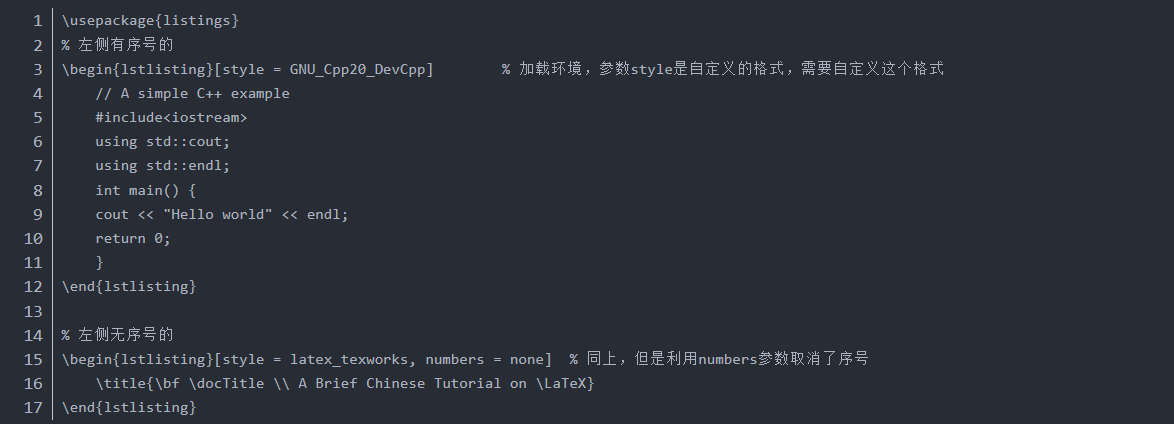
\includegraphics[height = 8cm, width = 18cm]{figure/1.png}		% 插入本地图片
\end{figure}
这里尤其要主要的是有关代码风格的问题,latex中默认是没有代码风格的,只显示黑白文字,因此需要自己设置,下面给出一些代码高亮的设置代码,方便后续使用:
\begin{enumerate}
\LaTeX 代码高亮\\
	\begin{lstlisting}[style = LaTeX_TeXworks]
	\definecolor{bgcolor_gray}{rgb}{0.9, 0.9, 0.9}
	\definecolor{deep_green}{rgb}{0, 0.5, 0}
	\lstdefinestyle{LaTeX_TeXworks}{
		language=[LaTeX]TeX,
		basicstyle=\ttfamily\small, % 设置基本字体样式
		backgroundcolor=\color{gray!10}, % 设置背景颜色
		morekeywords = {includegraphics, subcaptionbox, multirow},
		keywordstyle=\color{blue}, % 设置关键字颜色
		commentstyle=\color{green!50!black}, % 设置注释颜色
		stringstyle=\color{orange}, % 设置字符串颜色
		numbers=left, % 行号显示在左侧
		numberstyle=\tiny\color{gray}, % 设置行号字体样式和颜色
		stepnumber=1, % 行号递增步长
		numbersep=8pt, % 行号与代码之间的距离
		tabsize=4, % 制表符大小
		showspaces=false, % 是否显示空格
		showstringspaces=false, % 是否显示字符串中的空格
		captionpos=b, % 标题位置:底部
		breaklines=true, % 自动换行
		frame=tb, % 框架位置:上下
		framerule=0pt, % 框架宽度
		frameround=ftft, % 框架边角形状:上下左右
		framesep=3pt, % 框架与代码之间的距离
		aboveskip=10pt, % 代码与上方内容的距离
		belowskip=10pt, % 代码与下方内容的距离
		showtabs = false,
		extendedchars = true,
		inputencoding = utf8,	
	}	
	\end{lstlisting}
	
	\item C++代码高亮\\
	\begin{lstlisting}[style = LaTeX_TeXworks]
	%%% Tips: C++20关键字:alignas, alignof, and, and_eq, asm, atomic_cancel, atomic_commit, atomic_noexcept, auto, bitand, bitor, bool, break, case, catch, char, char8_t, char16_t, char32_t, class, compl, concept, const, consteval, constexpr, constinit, const_cast, continue, co_await, co_return, co_yield, decltype, default, delete, do, double, dynamic_cast, else, enum, explicit, export, extern, false, float, for, friend, goto, if, inline, int, long, mutable, namespace, new, noexcept, not, not_eq, nullptr, operator, or, or_eq, private, protected, public, reflexpr, register, reinterpret_cast, requires, return, short, signed, sizeof, static, static_assert, static_cast, struct, switch, synchronized, template, this, thread_local, throw, true, try, typedef, typeid, typename, union, unsigned, using, virtual, void, volatile, wchar_t, while, xor, xor_eq
	%%% 宏在morekeywords里不起作用,似乎是所有控制序列都被转义了
	\lstdefinelanguage[ISO]{C++20}{language = [ISO]C++, morekeywords = {alignas, alignof, atomic_cancel, atomic_commit, atomic_noexcept, char8_t, char16_t, char32_t, concept, consteval, constexpr, constinit, co_await, co_return, co_yield, decltype, noexcept, nullptr, reflexpr, requires, static_assert, synchronized, thread_local}}
	\lstdefinelanguage[GNU]{C++20}{language = [GNU]C++, morekeywords = {alignas, alignof, atomic_cancel, atomic_commit, atomic_noexcept, char8_t, char16_t, char32_t, concept, consteval, constexpr, constinit, co_await, co_return, co_yield, decltype, noexcept, nullptr, reflexpr, requires, static_assert, synchronized, thread_local}}
	\lstdefinelanguage[ANSI]{C++20}{language = [ANSI]C++, morekeywords = {alignas, alignof, atomic_cancel, atomic_commit, atomic_noexcept, char8_t, char16_t, char32_t, concept, consteval, constexpr, constinit, co_await, co_return, co_yield, decltype, noexcept, nullptr, reflexpr, requires, static_assert, synchronized, thread_local}}
	\lstdefinelanguage[Visual]{C++20}{language = [Visual]C++, morekeywords = {alignas, alignof, atomic_cancel, atomic_commit, atomic_noexcept, char8_t, char16_t, char32_t, concept, consteval, constexpr, constinit, co_await, co_return, co_yield, decltype, noexcept, nullptr, reflexpr, requires, static_assert, synchronized, thread_local}}
	%% C++20语法高亮
	\lstdefinestyle{GNU_Cpp20_DevCpp}{
		language = [GNU]C++20,
		captionpos = b,
		tabsize = 4,
		breaklines = true,
		showspaces = false,
		showtabs = false,
		frame = none,
		backgroundcolor = \color{bgcolor_gray},
		basicstyle = \CourierNew \SimSun,
		keywordstyle = \color{black} \bf,
		identifierstyle = \color{blue!50},
		commentstyle = \color{deep_green},
		numbers = left,
		numberstyle = \small,
		stepnumber = 1,
		firstnumber = 1,
		extendedchars = true,
		inputencoding = utf8,
	}	
	\end{lstlisting}
	
\end{enumerate}